\documentclass[11pt,a4paper]{amsart}
\usepackage[utf8]{inputenc}
\usepackage[T1]{fontenc}
\usepackage{lmodern}
\usepackage{amsmath,amssymb,amsthm}
\usepackage{booktabs}
\usepackage{graphicx}
\graphicspath{{figures/}}
\usepackage{xcolor}
\usepackage[margin=2.5cm]{geometry}
\usepackage[colorlinks=true,linkcolor=blue!50!black,citecolor=blue!50!black,urlcolor=blue!50!black]{hyperref}

\newtheorem{theorem}{Theorem}[section]
\newtheorem{proposition}[theorem]{Proposition}
\newtheorem{lemma}[theorem]{Lemma}
\theoremstyle{remark}
\newtheorem{remark}[theorem]{Remark}

\newcommand{\F}{\mathbb{F}}
\newcommand{\cS}{\mathcal{S}}
\numberwithin{equation}{section}
\emergencystretch=1.5em

\title[Explicit prescribed coefficients]{A note on the explicit theorem of Ha on irreducible polynomials with
prescribed coefficients}
\thanks{Code and data: \url{https://github.com/Ruqing1963/ha-explicit-constants-note}}
\author{Ruqing Chen}
\address{GUT Geoservice Inc., Montreal, Canada}
\email{ruqing@hotmail.com}
\date{November 2026}
\subjclass[2020]{Primary 11T06; Secondary 11T55, 11T23}
\keywords{irreducible polynomials, finite fields, prescribed coefficients, Hansen--Mullen conjecture, circle method}

\begin{document}

\begin{abstract}
Ha proved that there are irreducible polynomials of degree $n$ over $\F_q$ with $r$ prescribed coefficients in
arbitrary positions when $r\le(1/4-\epsilon)n$ and $q$ is large, and gave three explicit ranges of $(q,n,r)$. We
recompute the explicit constants of that paper. With the formulas as printed, the sufficient condition fails at the
boundary of two of the three ranges, and three steps of the argument need repair. We give a corrected criterion. It
recovers the first two explicit assertions (the second already for $n\ge71$ instead of $n\ge97$) and the third for
$q\ge3$; for $q=2$ it requires $n\ge81$ instead of $n\ge52$.
\end{abstract}

\maketitle

\section{Introduction}\label{sec:intro}

Ha \cite{Ha} proves, by the circle method of Hayes \cite{Hayes} and Pollack \cite{Pollack} combined with an idea of
Bourgain, that irreducible polynomials of degree $n$ with $r$ prescribed coefficients exist for $r\le(1/4-\epsilon)n$
and $q$ large, and for $r\le\delta n$ and all $q$ \cite[Theorem~1.1, Corollary~1.2]{Ha}. We have no objection to
these statements. The explicit Theorem~1.3 of \cite{Ha} asserts existence (a) for $n\ge8$, $q\ge16$,
$r\le n/4-\log_qn-1$; (b) for $q\ge5$, $n\ge97$, $r\le n/5$; (c) for all $q$, $n\ge52$, $r\le n/10$. Its proof
\cite[\S4]{Ha} consists of the numerical evaluation of a sufficient condition, and this is what we examine. We use
the notation of \cite{Ha}: $X=n$, $\hat X=q^X$, $\mathcal I$ is the set of prescribed positions, $r=|\mathcal I|$,
$\rho=r/X$, $\cS_{\mathcal I}(\alpha)$ and $\cS(\alpha)$ are the exponential sums over the prescribed set and over
the irreducibles, $C_{(x)}=x/(x-1)$, and $J=\lceil X/(r+1)\rceil$.

\begin{theorem}\label{thm:Ha}
Let $C_3,C_8$ be the constants of \cite[\S\S3--4]{Ha}.
\begin{enumerate}
\item[(a)] With the formulas as printed, the sufficient condition $1>C_8q^{-C_2/\rho}+q^{-B}$ of \cite[\S4]{Ha} fails
at $(q,\rho,B)=(16,\frac14,1)$ and at $(5,\frac15,2)$: its right-hand side is $1.3004$ and $1.0121$, not $0.994$ and
$0.884$. The stated values $C_8\le8.552$ and $C_8\le12.335$ are in fact $11.376$ and $14.212$.
\item[(b)] Three steps of the argument need repair: inequality \textup{(13)}, the replacement of
$\lceil n/(r+1)\rceil$ by $1/\rho$, and the treatment of denominators divisible by $T$, to which
\cite[Lemmas~2.6, 2.7]{Ha} do not apply.
\item[(c)] A corrected criterion (Proposition~\ref{prop:restored}) gives: an irreducible polynomial of degree $n$ with
$r$ prescribed coefficients (constant term not prescribed to $0$) exists if $q\ge16$ and
$1\le r\le n/4-\log_qn-1$; if $q\ge5$, $n\ge71$ and $r\le n/5$; if $q\ge3$, $n\ge21$ and $r\le n/10$; and if $q=2$,
$n\ge81$ and $r\le n/10$.
\end{enumerate}
\end{theorem}

Part (c) recovers \cite[Theorem~1.3]{Ha} except for $q=2$, $52\le n\le80$, $r\le n/10$, which our criterion does not
reach. Part (a) is proved in Section~\ref{sec:printed}, part (b) in Section~\ref{sec:repair} and part (c) in
Section~\ref{sec:criterion}. The asymptotic results of \cite{Ha} are not affected. The numerical statements are
checked by the script \texttt{code/verify\_ha\_audit.py} (pure Python).

\section{The constants as printed}\label{sec:printed}
In \cite{Ha}, $C_1=\kappa\le2/(1+\rho)$, $C_2=1-2C_1\rho$,
\[
C_3=C_{(q^{C_2})}\Bigl(e+e^\gamma+\frac{e^\gamma}{q\log q}\Bigr),\qquad
C_4\log_qJ+C_5=e^\gamma C_{(q^{C_2})}\Bigl(\log_qJ+1+\frac1{J\log q}\Bigr),
\]
$C_8=C_{(q)}\max\{C_3,\,C_4\log_q(1/\rho)+C_5\}$, and the sufficient condition is
$1>C_8q^{-C_2/\rho}+q^{-B}$ for $r\le X/4-\log_qX-B$. Table~\ref{tab:ha} evaluates these formulas at the boundary
values of $\rho$, with $C_1=2/(1+\rho)$, which is the value behind the exponent $1/\rho-4/(\rho+1)=C_2/\rho$ of
\cite[Theorem~1.1]{Ha}. The exponents $q^{C_2/\rho}$ agree with those used in \cite{Ha}; the values of $C_8$ do
not, and in the first two cases the condition fails. With the printed formulas it holds at $\rho=1/4$, $B=1$ only for
$q\ge23$, and at $\rho=1/5$, $B=2$ only for $q\ge7$.

\begin{table}[ht]
\centering
\caption{The constants of \cite[\S4]{Ha} recomputed from the printed formulas; ``RHS'' is
$C_8q^{-C_2/\rho}+q^{-B}$.}\label{tab:ha}
\small
\begin{tabular}{@{}rrrrrrrrrr@{}}
\toprule
$q$ & $\rho$ & $B$ & $C_2$ & $C_{(q^{C_2})}$ & $C_3$ & $C_8$ & $C_8$ in \cite{Ha} & RHS & RHS in \cite{Ha}\\
\midrule
$16$ & $1/4$ & $1$ & $0.2000$ & $2.3493$ & $10.6649$ & $11.3758$ & $8.552$ & $1.3004$ & $0.994$\\
$5$ & $1/5$ & $2$ & $0.3333$ & $2.4085$ & $11.3698$ & $14.2122$ & $12.335$ & $1.0121$ & $0.884$\\
$2$ & $1/10$ & $2$ & $0.6364$ & $2.8037$ & $16.2171$ & $44.6052$ & $42.342$ & $0.7917$ & $0.764$\\
\bottomrule
\end{tabular}
\end{table}

\section{Three steps that need repair}\label{sec:repair}
\emph{(i) Inequality \textup{(13)}.} From $\log_qj\le\log_qA+(j-A)/(A\log q)$ one gets
\[
\sum_{j\ge A}\frac{\log_qj}{q^{C_2j}}\le\Bigl(\log_qA+\frac1{(q^{C_2}-1)A\log q}\Bigr)\frac{C_{(q^{C_2})}}{q^{C_2A}},
\]
with the extra factor $1/(q^{C_2}-1)$, which exceeds $1$ when $q^{C_2}<2$.

\emph{(ii) $J$ versus $1/\rho$.} The decay obtained in \cite[\S3]{Ha} is $q^{-C_2J}$ with $J=\lceil X/(r+1)\rceil$,
and $J$ can be smaller than $1/\rho=X/r$ (for $X=97$, $r=19$: $J=5<5.1$; for small $r$ the difference is large).

\emph{(iii) Denominators divisible by $T$.} \cite[Lemma~2.6]{Ha} is stated and proved for $(aT,g)=1$: the shift
$a\mapsto T^{j_*}a$ must be a bijection of the reduced residues modulo $g$. In \cite[(14)]{Ha} the terms with
$g=Tg_0$ are included without argument. Also, for $g=Tg_0$ the proof of \cite[Lemma~2.7]{Ha} gives only
$|g_0|\ge q^{J-1}$ when the run of vanishing coefficients starts at the position $T^{-1}$. The following lemma
replaces both.

\begin{lemma}\label{lem:Tg}
Let $g_0$ be monic and prime to $T$, $c$ prime to $g_0$, and $b\in\F_q^\times$.
\begin{enumerate}
\item[(a)] If $0\in\mathcal I$, then $\cS_{\mathcal I}(b/T+c/g_0)=\mathbf e(a_0b/T)\,\cS_{\mathcal I}(c/g_0)$.
\item[(b)] If $0\notin\mathcal I$, then $\sum_{b\ne0}|\cS_{\mathcal I}(b/T+c/g_0)|\le q\,|\cS_{\mathcal I^+}(c/g_0)|$,
where $\mathcal I^+=\mathcal I\cup\{0\}$.
\end{enumerate}
\end{lemma}

\begin{proof}
By \cite[(8)]{Ha}, $\cS_{\mathcal I}(\alpha)=q^{X-r}\mathbf e(\alpha T^X)\prod_{j\in\mathcal I}\mathbf e(a_jT^j\alpha)$
if $\alpha_{-j-1}=0$ for all $j\notin\mathcal I$, $0\le j<X$, and $\cS_{\mathcal I}(\alpha)=0$ otherwise. Adding
$b/T$ changes only the coefficient $\alpha_{-1}$, by $b$. If $0\in\mathcal I$ the vanishing conditions are unchanged
and the product changes by $\mathbf e(a_0b/T)$. If $0\notin\mathcal I$, the condition $\alpha_{-1}=0$ holds for at
most one $b$, and the remaining conditions are those of $\mathcal I^+$, whose sum has modulus $q^{X-r-1}$.
\end{proof}

Since $\mu(Tg_0)/\phi(Tg_0)=-\mu(g_0)/((q-1)\phi(g_0))$ and $\sum_{b\ne0}\mathbf e(-a_0b/T)\in\{q-1,-1\}$, part (a)
shows that for $0\in\mathcal I$ the terms with $g=Tg_0$ equal those with $g=g_0$ times $-1$ (if $a_0=0$) or
$1/(q-1)$ (if $a_0\ne0$): this is the singular series $\mathfrak S$ of \cite[(2)]{Ha}, and it justifies the factor
$C_{(q)}$ in $C_8$ in that case. For $0\notin\mathcal I$, part (b) gives the factor $1/(q-1)$ at the cost of
replacing $\mathcal I$ by $\mathcal I^+$.

\section{A corrected criterion}\label{sec:criterion}
For $0\le\rho<1/3$ let $c_2(\rho)=(1-3\rho)/(1+\rho)$, let $w_q(j)=e$ for $j\le q$ and
$w_q(j)=e^\gamma(\log_qj+1)$ for $j>q$, and
\[
\Sigma_q(\rho,J)=\sum_{j\ge J}w_q(j)\,q^{-c_2(\rho)j}.
\]

\begin{proposition}\label{prop:restored}
Let $q$ be a prime power, $\mathcal I\subseteq\{0,\dots,n-1\}$ with $|\mathcal I|=r$ and $3(r+1)<n$, and let
$a_j\in\F_q$ for $j\in\mathcal I$, with $a_0\ne0$ if $0\in\mathcal I$. If
\begin{equation}\label{eq:crit}
\Sigma_q\Bigl(\frac rn,\Bigl\lceil\frac n{r+1}\Bigr\rceil\Bigr)
+\frac1{q-1}\,\Sigma_q\Bigl(\frac{r+1}n,\Bigl\lceil\frac n{r+2}\Bigr\rceil\Bigr)
+\frac{n\,q^{\,r-n/4}}{1-2q^{-n/2}}<1,
\end{equation}
then there is a monic irreducible polynomial of degree $n$ whose coefficient of $T^j$ is $a_j$ for all
$j\in\mathcal I$. The proof uses \cite[Lemmas~2.1--2.4, 2.8]{Ha} and \cite[Lemma~2.7]{Ha} for denominators prime
to $T$.
\end{proposition}

\begin{proof}
Let $N=\int_{\mathbf T}\cS(\alpha)\overline{\cS_{\mathcal I}(\alpha)}\,d\alpha$ be the number sought. On the Farey arc
around $a/g$, \cite[Lemma~2.8]{Ha} gives $\cS(a/g+\gamma)=\mu(g)\phi(g)^{-1}\pi_q(X)\mathbf e(\gamma T^X)
\mathbf 1_{|\gamma|<1/\hat X}+R$ with $|R|\le\hat X^{3/4}$. Since $\int_{\mathbf T}|\cS_{\mathcal I}|=1$
\cite[Lemma~2.4]{Ha}, the terms $R$ contribute at most $\hat X^{3/4}$ in total, on major and minor arcs together, and
\[
N=\frac{\pi_q(X)}{\hat X}\sum_{a/g}\frac{\mu(g)}{\phi(g)}\,\overline{\cS_{\mathcal I}(a/g)}+\theta\hat X^{3/4},\qquad|\theta|\le1,
\]
the sum being over reduced fractions with $\deg g\le X/2$. The terms $g=1$ and $g=T$ give
$\mathfrak S\,\pi_q(X)q^{-r}$ with $\mathfrak S\ge1$ (namely $\mathfrak S=q/(q-1)$ if $0\in\mathcal I$, and
$\mathfrak S=1$ if $0\notin\mathcal I$, since then $\cS_{\mathcal I}(b/T)=0$ for $b\ne0$); here we used
$\cS_{\mathcal I}(a/g+\gamma)=\mathbf e(\gamma T^X)\cS_{\mathcal I}(a/g)$ for $|\gamma|<1/\hat X$. Let
\[
E(\mathcal I)=q^{-(X-r)}\sum_{g_0}\frac{\mu(g_0)^2}{\phi(g_0)}\sum_{(c,g_0)=1}|\cS_{\mathcal I}(c/g_0)|,
\]
over monic $g_0\ne1$ prime to $T$ with $\deg g_0\le X/2$. By Lemma~\ref{lem:Tg} the remaining terms are bounded by
$\pi_q(X)q^{-r}\mathfrak S\,E(\mathcal I)$ if $0\in\mathcal I$, and by
$\pi_q(X)q^{-r}\bigl(E(\mathcal I)+E(\mathcal I^+)/(q-1)\bigr)$ if $0\notin\mathcal I$.

To bound $E(\mathcal I)$: by \cite[Lemma~2.7]{Ha} only $\deg g_0\ge J=\lceil X/(r+1)\rceil$ occurs. Fix $j$ with
$J\le j\le X/2$. Choose a window of $2j$ consecutive positions in $\{0,\dots,X-1\}$ containing at most
$\kappa\rho\cdot2j$ elements of $\mathcal I$, with $\kappa\le2/(1+\rho)$: if $2j$ divides $X$ one may take
$\kappa=1$; if $X/2j>2$, the $\lfloor X/2j\rfloor$ disjoint windows give $\kappa\le3/2\le2/(1+\rho)$; and if
$1<X/2j<2$, the two extreme windows overlap in $4j-X$ positions and contain together at most
$r+\min(r,4j-X)$ elements, which gives $\kappa\le2/(1+\rho)$ in both cases. As in the proof of
\cite[Lemma~2.6]{Ha}, shifting by the window and using that the fractions $c/g_0$ with $\deg g_0\le j$ are
$q^{-2j}$-separated,
\[
\sum_{\deg g_0\le j}\ \sum_{(c,g_0)=1}|\cS_{\mathcal I}(c/g_0)|\le\hat Xq^{-r}q^{2j\kappa\rho}
\le\hat Xq^{-r}q^{\,j(1-c_2(\rho))}.
\]
With $|g_0|/\phi(g_0)\le w_q(\deg g_0)$ \cite[Lemma~2.3]{Ha}, this gives
$E(\mathcal I)\le\Sigma_q(\rho,J)$, and likewise $E(\mathcal I^+)\le\Sigma_q((r+1)/n,\lceil n/(r+2)\rceil)$. Finally
$\pi_q(X)\ge\hat XX^{-1}(1-2\hat X^{-1/2})$ \cite[Lemma~2.2]{Ha}, so $N>0$ as soon as
$1-E(\mathcal I)-E(\mathcal I^+)/(q-1)>Xq^{r-X/4}/(1-2q^{-X/2})$.
\end{proof}

The left side of \eqref{eq:crit} is nonincreasing in $q$ and nondecreasing in $r$. Table~\ref{tab:restored} gives,
for hypotheses of the form $(r+1)/n\le\rho^*$, $\lceil n/(r+2)\rceil\ge J^*$ and $r\le n/4-\log_qn-B$, the least
$q_0$ such that the resulting bound $C_{(q)}\Sigma_q(\rho^*,J^*)+q^{-B}/(1-2q^{-4})$ is less than $1$ for all prime
powers $q\ge q_0$.

\begin{table}[ht]
\centering
\caption{Least $q_0$ for the corrected criterion, and the value of the bound at $q_0$.}\label{tab:restored}
\small
\begin{tabular}{@{}ccrrrr@{}}
\toprule
$\rho^*$ & $J^*$ & $q_0$ ($B=1$) & bound & $q_0$ ($B=2$) & bound\\
\midrule
$1/4$ & $4$ & $16$ & $0.8040$ & $13$ & $0.9507$\\
$1/5$ & $5$ & $5$ & $0.9111$ & $5$ & $0.7506$\\
$1/6$ & $6$ & $4$ & $0.6138$ & $4$ & $0.4249$\\
$1/8$ & $8$ & $3$ & $0.4750$ & $3$ & $0.2472$\\
$1/10$ & $10$ & $3$ & $0.3573$ & $2$ & $0.8362$\\
\bottomrule
\end{tabular}
\end{table}

\begin{proof}[Proof of Theorem~\ref{thm:Ha}]
(a) is Table~\ref{tab:ha}, and (b) is the discussion above. For (c): let $q\ge16$ and $1\le r\le n/4-\log_qn-1$. Then
$(r+1)/n\le1/4$. For $r\ge2$, $n/(r+2)\ge4(r+1+\log_qn)/(r+2)>3$, so $J^*\ge4$, and the first line of
Table~\ref{tab:restored} applies. The case $r=1$ is the Hansen--Mullen conjecture, proved in \cite{Wan,HamMullen}.
For the other two families we evaluated the left side of \eqref{eq:crit} with $r=\lfloor n/5\rfloor$, $q=5$ and
with $r=\lfloor n/10\rfloor$, $q=2,3$, for all $n\le3000$: it is less than $1$ for $n\ge71$, for $n\ge81$ and for
$n\ge21$ respectively (at $q=2$, $n=52$ it equals $1.4662$). For $n>3000$ we have $\rho\le1/m$,
$\rho^*\le1/m+1/3000$ and $J,J^*\ge m$ with $m=5,10$, and \eqref{eq:crit} is bounded by $0.7119$, $0.5530$ and
$0.0156$ in the three cases. Monotonicity in $q$ and $r$ completes the proof.
\end{proof}

Table~\ref{tab:status} and Figure~\ref{fig:ha} summarise the outcome.

\begin{figure}[ht]
\centering
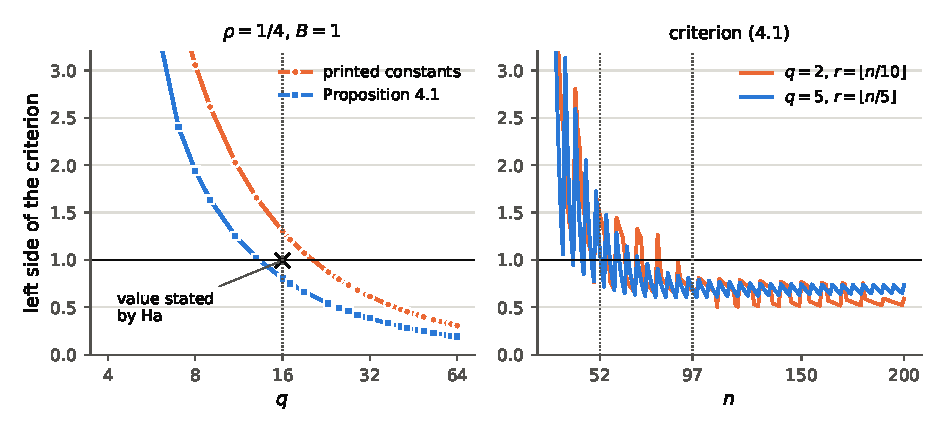
\includegraphics[width=0.95\textwidth]{fig_ha.pdf}
\caption{Left: the quantity that must be less than $1$, at $\rho=1/4$, $B=1$: with the constants as printed in
\cite{Ha} (it exceeds $1$ for $q<23$; the cross marks the value $0.994$ stated there for $q=16$), and the bound of
Proposition~\ref{prop:restored} with $\rho^*=1/4$, $J^*=4$. Right: the left side of \eqref{eq:crit} as a function
of $n$; it drops below $1$ for good at $n=81$ for $q=2$, $r=\lfloor n/10\rfloor$, and at $n=71$ for $q=5$,
$r=\lfloor n/5\rfloor$. The dotted lines mark the thresholds $52$ and $97$ of \cite{Ha}.}\label{fig:ha}
\end{figure} The gain over the printed constants comes from two points: the terms
with $\deg g_0>q$, which carry the weight $e^\gamma(\log_qj+1)$, are summed with their own decay $q^{-c_2j}$
instead of being bounded by the first term; and the error terms of the major and minor arcs are estimated
together, by $\hat X^{3/4}$ once. The repairs (i)--(iii) cost less than these gains, except for $q=2$.

\begin{table}[ht]
\centering
\caption{The three explicit assertions of \cite[Theorem~1.3]{Ha}.}\label{tab:status}
\small
\begin{tabular}{@{}lll@{}}
\toprule
assertion of \cite{Ha} & printed condition & criterion \eqref{eq:crit}\\
\midrule
$q\ge16$, $n\ge8$, $r\le n/4-\log_qn-1$ & fails for $q<23$ & holds\\
$q\ge5$, $n\ge97$, $r\le n/5$ & fails for $q=5$ & holds, already for $n\ge71$\\
all $q$, $n\ge52$, $r\le n/10$ & holds & holds for $q\ge3$, $n\ge21$;\\
 & & for $q=2$ only if $n\ge81$\\
\bottomrule
\end{tabular}
\end{table}

We have not examined \cite[Lemmas~2.3 and 2.8]{Ha}, nor the results of \cite{Hayes,Pollack} on which they rest; the
statements of this section are conditional on them in the form in which they are printed.

\begin{thebibliography}{9}

\bibitem{Ha} J. Ha, \emph{Irreducible polynomials with several prescribed coefficients}, Finite Fields Appl.
\textbf{40} (2016), 10--25.

\bibitem{HamMullen} K. H. Ham and G. L. Mullen, \emph{Distribution of irreducible polynomials of small degrees over
finite fields}, Math. Comp. \textbf{67} (1998), 337--341.

\bibitem{Hayes} D. R. Hayes, \emph{The expression of a polynomial as a sum of three irreducibles}, Acta Arith.
\textbf{11} (1966), 461--488.

\bibitem{Pollack} P. Pollack, \emph{Irreducible polynomials with several prescribed coefficients}, Finite Fields
Appl. \textbf{22} (2013), 70--78.

\bibitem{Wan} D. Wan, \emph{Generators and irreducible polynomials over finite fields}, Math. Comp. \textbf{66}
(1997), 1195--1212.

\end{thebibliography}

\end{document}
